\chapter{Microservice-Infrastruktur}
\label{chap:microserviceinfrastruktur}
Bevor man mit dem Programmieren der Anwendung anfangen kann,
gilt es einiges vorzubereiten. Dieses Kapitel beschäftigt sich
mit der Microservice-Infrastruktur der Gesamtanwendung. Hier geht
es um das Aufsetzen einer agilen Infrastruktur, die den
stetigen Auslieferungsprozess der Software ermöglicht. 
In \Cref{chap:qualitaetssicherung} geht es um Methoden und Verfahren,
die die Qualität der Software sicherstellen. Erst nach der Erstellung
der Microservice-Infrastruktur sowie der Automatisierung von
Qualitätssicherungsprozessen, kann mit der Programmierung der
Anwendung begonnen werden.

Das Kapitel Microservice-Infrastruktur ist wie folgt gegliedert:
In \Cref{sec:continuousdelivery} befasst sich die Arbeit mit
dem stetigen Softwareauslieferungsprozess, bekannt als Continuous Delivery.
In \Cref{sec:monorepoundsubmodules} wird die Aufteilung der Versionsverwaltung
in einzelne Aufbewahrungsorte diskutiert. In \Cref{sec:infrastruktur}
wird die Infrastruktur der Gesamtanwendung geschildert. Hier geht es
um Technologien, die das Auslieferungsverfahren sowie die Benutzung
der Anwendung in Produktion ermöglichen. In \Cref{sec:systemdesign}
geht es um die Gestaltung der Anwendung selbst. Hier werden die einzelnen,
für die Anwendung nötigen Komponenten erörtert und definiert. Dabei
wird auf die Frage des Tech-Stacks der einzelnen Services geklärt.
In \Cref{sec:pipelinedesign} geht es um die Pipeline, also den Auslieferungsprozess
selbst. Hier werden Vorkehrungen getroffen, um diesen zu ermöglichen.

\section{Continuous Delivery}
\label{sec:continuousdelivery}
Continuous Delivery (CD ist das Verfahren, Software in einem stetigen Zyklus auszuliefern.
Neue Technologien, wie die Containervirtualiserungssoftware Docker,
die im März 2013 von dotCloud ins Leben gerufen wurde \cite{DockerAbout2014}, vereinfachen
den stetigen Softwareauslieferungsprozess enorm. So kann man in einem automatisierten
Auslieferungsprozess, Images bauen, diese testen und selbige nach erfolgreichem
Bestehen der Tests in der Produktion verwenden. Eberhard Wolff schreibt über das Ziel von Docker in
seinem Buch "Continuous Delivery" folgendes: "Das Ziel von Docker ist es, Container für die
Distribution von Software zu nutzen. Im Vergleich zu normalen Prozessen trennen Linux-Container
einzelne Anwendungen viel besser voneinander, wenn es darum geht, die Software auf einem anderen
System zu installieren. Docker bietet ein Repository für Images an, so dass eine Vielzahl
von Servern mit identischen Images betrieben werden können."\cite[S. 56]{ContinuousDeliveryWolff}
Somit kann sichergestellt werden, dass die Software und deren Umgebung in der Testing-Stage
sowie in Produktion die selbe ist. Immer mehr Anbieter stellen CI-Werkzeuge zur Verfügung,
die es ermöglichen eine CI/CD-Pipeline anhand einer YML-Datei aufzuziehen. So bieten nun
neben Travis CI, CircleCI und Jenkins auch Versionsverwaltungshosts wie Github und
Gitlab CI-Werkzeuge zur Verfügung. \footnote{Github bietet seit 13. November 2019 eigene CI/CD-Werkzeuge an \cite{GithubCIToolsHeise}}


\section{Monorepo und Submodules}
\label{sec:monorepoundsubmodules}
% Git submodules

\section{Infrastruktur}
\label{sec:infrastruktur}

\subsection{Gitlab CE}
\label{subsec:gitlabce}
% Die Unabhängigkeit gegenüber einzelner Unternehmen
\subsection{Gitlab Runner}
\label{subsec:gitlabrunner}

\subsection{Docker Registry}
\label{subsec:dockerregistry}

\subsection{Hetzner Cloud}
\label{subsec:hetznercloud}

\section{Systemdesign}
\label{sec:systemdesign}

% Wahl der Technologien, Tech-Stack?
% Anforderungen an die Technologien
% Umfeld etc
% Geschwindigkeit der Entwicklung
\begin{figure}
    \label{figure:microserviceinfrastruktur}
    \begin{center}
    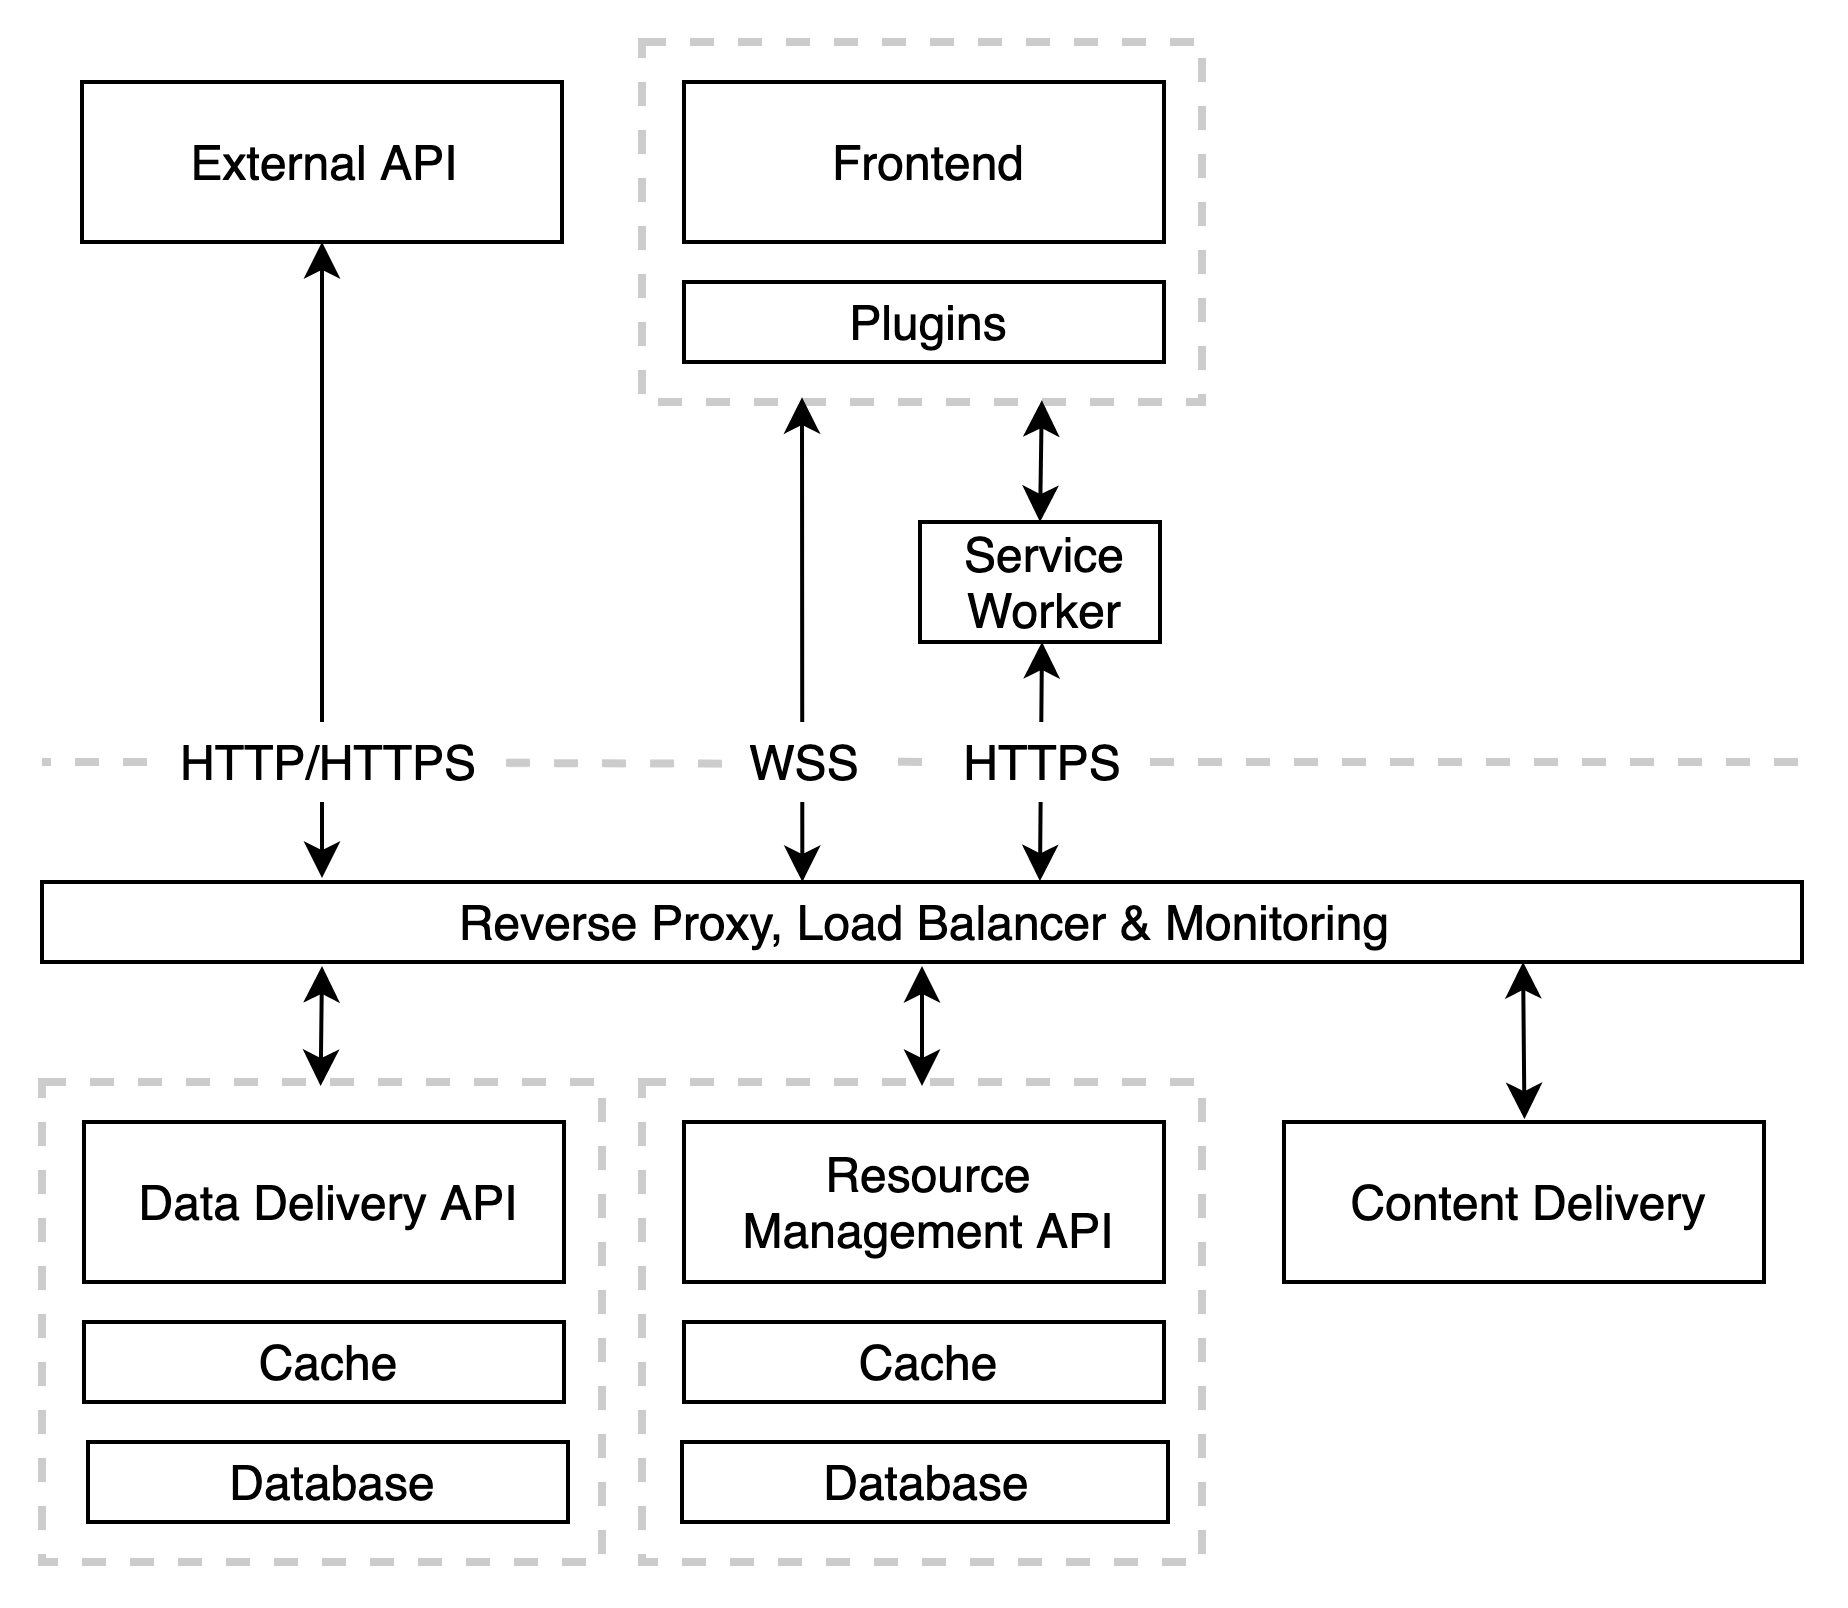
\includegraphics[scale=0.2]{img/abbildungen/MicroserviceInfrastruktur}
    \end{center}
    \caption{Übersicht über die Microservice-Infrastruktur}
\end{figure}

\subsection{Reverse Proxy}
\label{sec:reverseproxy}

\subsection{Load Balancer}
\label{sec:loadbalancer}

\subsection{Inhaltsauslieferung}
\label{sec:inhaltsauslieferung}

%% compression
% CDM

\subsection{Monitoring}
\label{sec:monitoring}

\subsection{Wartung}
\label{sec:wartung}
% clean up von server und docker setup

\section{Pipeline Design}
\label{sec:pipelinedesign}

\subsection{Umgebungsvariablen}
\label{subsec:umgebungsvariablen}

\subsection{Stages}
\label{subsec:stages}
% Continuous Integration mit Gitlab

\subsection{Docker Compose Setup}
\label{subsec:dockercomposesetup}

\subsection{Health-Checks}
\label{subsec:healthcheck}
In Microservice-Infrastrukturen sind die einzelnen Services eng miteinander verknüpft
und voneinander abhängig. Um die Verfügbarkeit sicherzustellen, werden auf
Serviceebene Healthcheckendpunkte bereitgestellt. Diese spiegeln den aktuellen
Gesundheitszustand des jeweiligen Dienstes wieder. Ein Healthcheckendpunkt
ist speziell dann nützlich, wenn ein Dienst oder ein Verfahren von einem anderen
abhängig ist. So ist beispielsweise die Backendapi von der Datenbank
abhängig. Andererseits ist der Frontenddienst sowie das Apitestverfahren
in der Buildpipeline von der Backendapi abhängig. 

\begin{listing}
    \label{lst:healthcheck}
    \inputminted{sh}{snippets/sh/healthcheck.sh}
    \caption{Healthcheckbeispiel in der Gitlab CI}
\end{listing}

